%!TEX root = ../Physik I.tex

\section{Einleitung} % (fold)
	\emphequation{align*}{
		\Div \vec E &= 0 \\
		\rot \vec E &= -\Part{\vec B}{t} \\
		\Div \vec B &= 0 \\
		c^2 \rot \vec B &= \Part{\vec E}{t}
	}
% section: Einleitung (end)
\section{Spezielle Relativitätstheorie} % (fold)
	\subsection{Einstein'schen Postulate} % (fold)
		\begin{tightitemize}
			\item Die physikalischen Gesetze haben dieselbe Form in allen Inertialsystemen
			\item Die Geschwindigkeit elektromagnetischer Wellen im Vakuum ist dieselbe in allen Inertialsystemen
		\end{tightitemize}
	% subsection: Einstein'schen Postulate (end)
	\subsection{Lorentz-Transformation} % (fold)
		\begin{center}
			%!TEX root = ../Physik I.tex

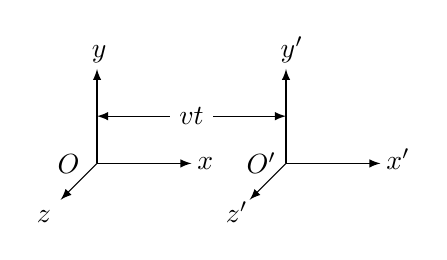
\begin{tikzpicture}[>=latex,scale=1.2]
	\begin{scope}
		\draw[->] (0,0) -- (xyz cs:x=1) node[right,xshift=-.5mm,yshift=.5mm]{$x\phantom{'}$};
		\draw[->] (0,0) -- (xyz cs:y=1) node[above,xshift=.75mm,yshift=-.5mm]{$y\phantom{'}$};
		\draw[->] (0,0) -- (xyz cs:z=1) node[below left,xshift=1mm,yshift=1mm]{$z\phantom{'}$};
		\draw (0,0) node[left]{$O\phantom{'}$};
	\end{scope}
	\begin{scope}[xshift=2cm]
		\draw[->] (0,0) -- (xyz cs:x=1) node[right,xshift=-.5mm,yshift=.5mm]{$x'$};
		\draw[->] (0,0) -- (xyz cs:y=1) node[above,xshift=.75mm,yshift=-.5mm]{$y'$};
		\draw[->] (0,0) -- (xyz cs:z=1) node[below left,xshift=1mm,yshift=1mm]{$z'$};
		\draw (0,0) node[left]{$O'$};
	\end{scope}
	\draw[<->] (0,.5) -- (2,.5) node[pos=.5,fill=white]{$vt$};
\end{tikzpicture}
		\end{center}
		\begin{align*}
			x &= \gamma(x' + vt') \\
			y &= y' \\
			z &= z' \\
			t &= \gamma\parens{t' + \frac{v x'}{c^2}} \\
			\gamma &= \frac{1}{\sqrt{1- \nicefrac{v^2}{c^2}}} = \frac{1}{\sqrt{1-\beta^2}}
		\end{align*}
	% subsection: Lorentz-Transformation (end)
	\subsection{Längenkontraktion} % (fold)
		Ein Beobachter im Ruhesystem misst eine andere Länge als ein Beobachter im
		bewegten System.
		
		Stab im ruhenden System mit Länge
		\begin{equation*}
			L_0 = x_2 - x_1
		\end{equation*}
		Im bewegten System:
		\begin{equation*}
			L = x_2' - x_1' = (x_2 - x_1) \sqrt{1-\beta^2} - v t_2' + v t_1'
		\end{equation*}
		Nur sinnvoll wenn $t_1' = t_2'$:
		\begin{equation*}
			L = L_0 \sqrt{1-\beta^2} = L_0 \sqrt{1-\nicefrac{v^2}{c^2}}
		\end{equation*}
	% subsection: Längenkontraktion (end)
	\subsection{Zeitdilatation} % (fold)
		Zwei Ereignisse finden im bewegten System statt im Zeitintervall
		\begin{equation*}
			\Delta t' = t_2' - t_1'
		\end{equation*}
		
		Im ruhenden System ergibt das:
		\begin{equation*}
			\Delta t = t_2 - t_1 = \frac{t_2' + x_2' \nicefrac{v}{c^2}}{\sqrt{1-\beta^2}}
			- \frac{t_1' + x_1' \nicefrac{v}{c^2}}{\sqrt{1-\beta^2}}
		\end{equation*}
	% subsection: Zeitdilatation (end)
% section: Spezielle Relativitätstheorie (end)
\section{Doppler-Effekt} % (fold)
	\subsection{Klassische Doppler-Effekt} % (fold)
		Quelle und Empfänger bewegen sich weg voneinander:
		\begin{equation*}
			\nu' = \nu \parens{1-\frac{v}{c}}
		\end{equation*}
		Quelle und Empfänger bewegen sich zueinander:
		\begin{equation*}
			\nu' = \nu \parens{1+\frac{v}{c}}
		\end{equation*}
		\begin{itemize}
			\item[$\nu$:] Frequenz des Senders
			\item[$\nu'$:] Vom Beobachter erfahrene Frequenz
		\end{itemize}
	% subsection: Klassische Doppler-Effekt (end)
	\subsection{Relativistische Doppler-Effekt} % (fold)
		Wellengleichung ist im gestrichenen genau gleich wie im ungestrichenen System.
		
		Für die Frequenzverschiebung ergibt sich die \textbf{relativistische Dopplerformel}:
		\begin{align*}
			\nu' &= \nu \frac{1-\beta}{\sqrt{1-\beta^2}}
			= \nu \frac{\sqrt{1-\beta}}{\sqrt{1+\beta}} \\
			&= \nu \parens{
				1 - \beta + \half \beta^2 - \cdots
			} \\
			&= \nu \parens{
				1 - \frac v c + \half \frac{v^2}{c^2} - \cdots
			}
		\end{align*}
	% subsection: Relativistische Doppler-Effekt (end)
% section: Doppler-Effekt (end)